\section{Cloud Storage}

\subsection{Storing Data}

Relational databasis management systems fit on a single machine. This is a problem if we deal with Petabytes of data, which cannot be stored on one machine.
When dealing with large amounts of data, the majority of the properties stay the same. A few things that change include:
\begin{itemize}
    \item no tabular integrity anymore
    \item no domain integrity anymore
    \item no atomic integrity anymore
    \item $2^{nd}$/$3^{rd}$/Boyce-Codd normal form are lost
    \item new heterogeneous data: data that does not fulfill domain integrity (it may not even have a schema!) and also not relational integrity.
    \item new nested data: data that is not in first normal form
    \item new denormalized data
\end{itemize}
This new domain is called NoSQL universe.

\subsection{The technology stack}
We go from a monolithic relational database to a modular "Big Data" technology stack.

\begin{figure}[h]
    \centering
    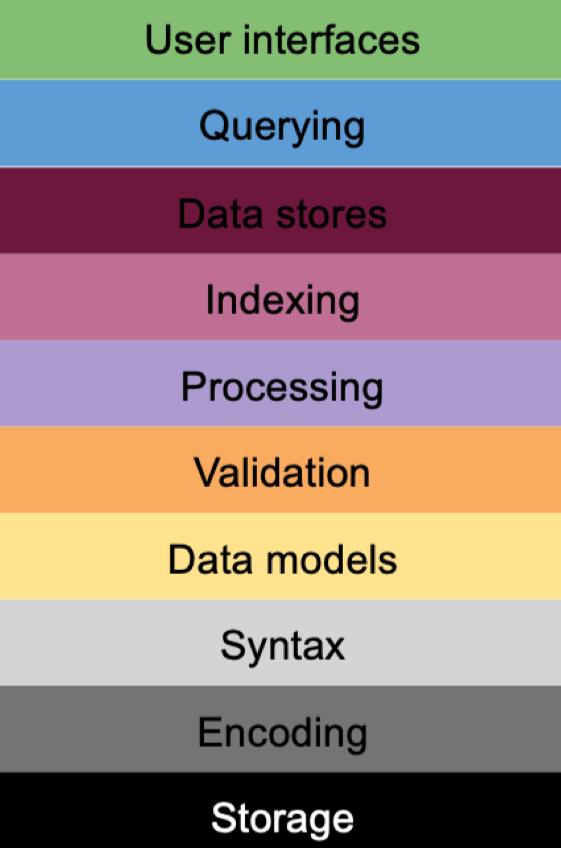
\includegraphics[width=0.35\textwidth]{Figures/Technology_Stack.jpeg}
    \caption{The Technology Stack}\label{fig:TechStack}
\end{figure}

\subsection{Databases vs. Data lakes}

In a traditional database, data can be imported into the database (this is called ETL, for Extract-Transform-Load).
In a data lake, you read directly from a file system and queried in place (in situ) by a data processing engine. This paradigm gained a lot of popularity in the past. It is slower, however users can start querying their data without the effort of ETLing.


\subsection{From your laptop to a data center}

Data are locally stored on SSDs. Files are split in blocks. This is to optimize the balance between throughput and latency.
A disk can be made available via the network (LAN for Local Area Network) and shared with other people. There exists a larger network (WAN for Wide Area Netowrks), however it is difficult to scale concurrent access and problems can arise already when two people work on a file at the same time.
Another scalability problem is that a local file system can easily support 1000 files or even 1,000,000 files, but can hardly make it to billions of files.
One approach for large scales, namely object storage, is to:
\begin{itemize}
    \item throw away the hierarchy: there are no directories
    \item make the metadata flexible: attribute can idffer from file to file (no schema)
    \item use a very simple, if not trivial, data model: a flat list of files (called objects) identified with an identifier (ID). Blocks are not exposed to the user, i.e., an object is a blackbox.
    \item use a large number of cheap machines rather than some "supercomputers"
\end{itemize}

\subsection{Scale up vs. scale out}

\paragraph{Scaling up} means, that one can buy bigger machines with more memory, more or faster CPU cores, a larger disk, etc.

\paragraph{Scaling out} means, one can buy more similar machines and share the work across them. Scaling out is much cheaper than scaling up.

\paragraph{Third way: Optimizing your code} By writing very efficient code, one can dodge having to scale out or up.

\subsubsection{Data centers}
There are tens of thousands of machines in a datacenter. The upper bound of number of machines is roughly 100,000 machines, because beyond this number, coolings starts to become critical. Furtheremore, the energy consumption is roughly the same as an airport.

There are roughly 1-200 cores per server, 1-30 TB of local storage per server, 16GB-6TB of RAM per server, 1-100 Gbits/s network bandwidth for a server.

Machines are flat and are stacked upon each other. This tower is called a \textit{Rack}.


\subsection{Object stores}

\subsubsection{Amazon S3}

It is a global cloud servive. There are buckets with bucket IDs and there are objects (files) inside the buckets (also labeled with IDs). The maximal size of a file is 5 TB and there are no buckets in buckets, and you can have a maximum of 100 buckets per user.

\paragraph{Dataset Hosting}
It may cause problems if you want to down- or upload large files to a cloud. It is therefore useful, to devide the data into chuncks and then up- or download the data chunkwise.

\paragraph{Storage Class}
There are three classes:
\begin{itemize}
    \item Standard: high availability
    \item Standard - Infrequent Access: Less availability, cheaper storage, cost for retrieving
    \item Amazon Glacier: Low-cost Hours to GET
\end{itemize}

\subsubsection{Azure Blob Storage}
Azure is also a cloud system service, with almost the same properties as Amazon S3. Some differences include:
\begin{itemize}
    \item Architecture is publicly documented
    \item Objects are identified with three instead of 2 IDs: An Account, a Container and a Blob
    \item More detail is exposed to the user. It exposes that objects are devided in several blocks more prominently than Amazon S3.
    \item It differentiates between Block Blobs, Append Blobs (for logging), and Page Blobs (for storing and accessing the memory of virtual machines).
    \item The maximum sizes are different and go from 195GB for an Append Blob to 190.7 TB for a Block Blob, and 8 TB for a page.
\end{itemize}

Azure Blob is organized in so-called storage stamps, located in various data centers worldwide. Each storage stamp consists of 10 to 20 racks, wich each rack containing around 18 storage nodes (the disk+servers). In all, a storage stamp can store up to ca. 30 PB of data. However, a storage stamp will not be filled more than 80\% of its total capacity in order to avoid being full: if a storage stamp reaches capacity, then some data is going to be reallocated to another storage stamp in the background. And if there are not enough storage stamps, well new racks will need to be purchased and installed at the location that make the most sense.

\paragraph{Storage Replication}
There are two types of storage replication.
\begin{itemize}
    \item Intra-stamp replication (synchronous): you can only work with the data if it has been stored twice or three times.
    \item Inter-stamp replication (asynchronous): communication across datacenters. You do not have to wait in this process. You can already work on other problems while the files get transfered.
\end{itemize}

\subsection{Guarantees and service level}

\subsubsection{Service Level Agreements}

Customers of cloud services one something in exchange for their money. These are:

\paragraph{Durability} The amount of information lost, each year, e.g. loss of 1 in $10^{11}$ object per year corresponds to a durability of $99.999999999\%$

\paragraph{Availability} If a service is available $99.99\%$ of the time, the server will be down less than 1h per year.

\paragraph{Response time} E.g. 99.9\% of the requests will be served in less than 300ms.


\subsubsection{The CAP theorem}

In order to scale out, many distributed systems have to make a compromise on the transactional guarantees that they offer. The CAP theorem is an impossibility triangle. A system cannot guarantee at the same time
\begin{itemize}
    \item (atomic) Consistency: at any point in time, the same request to any server returns the same result, in other words, all nodes see the same data
    \item Availability: the system is available for requests at all times (SLA with very high availability)
    \item Partition tolerance: the system continues to function even if the network linking its machines is occasionally partitioned.
\end{itemize}

\subsection{REST APIs}

REST stands for Representational State Transfer. ("HTTP done right"). A resource is refered to with a so-called URI (Uniform Resource Identifier), e.g. http://www.example.com/api/collection/foobar?id=foobar\#head where
\begin{itemize}
    \item http is the scheme
    \item //www.example.com is the authority
    \item /api/collection/foobar is the path
    \item ?id=foobar is the query
    \item \#head is the fragment
\end{itemize}
Example for Amazon S3:
http://bucket.s3.eu-west-1.amazonaws.com for a bucket and http://bucket.s3.eu-west-1.amazonaws.com/object-name for an object.

A client can act on resources by invoking methods, with an optional body. The most important methods are
\begin{itemize}
    \item GET (without a body): this method returns a representation of the resource in some format. GET should have no side effects.
    \item PUT: create or update a resource from a representation of a newer version of it, in some format. PUT has the side effect that a subsequent GET asking for the same format should return the same representation. PUT is idempotent, in that calling PUT with the same resource and body is identical to callint it just once.
    \item DELETE (without a body): this method deletes a resource. DELETE has the side effect that a subsequent GET asking for a representation of the resource should fail with a not-found (404) error.
    \item POST: this method is a blank check, in that it acts on a resource in any way the data store seems fit. The behaviour, of course, should be publicly documented. A typical use of POST is to create new resources but letting the REST server pick a resource URI for this new resource.
\end{itemize}

\subsection{Summary}

How to scale out?
Simplify the model, Buy cheap hardware, remove schemas